\documentclass[../zavrsni.tex]{subfiles}

\begin{document}

\sloppy

\justifying

\section{Generiranje skupova testnih zadataka}

%\subsection{UUniFast algoritam}

%\subsection{Generiranje vrijednosti perioda}

%\subsection{Implementacija generatora testnih zadataka}

Generiranje skupova zadataka implementirano je u datoteci \texttt{taskSetGenerator.c}. U strukturi \texttt{periodic\_task} sadržane su sve 
informacije potrebne za opis pojedinog zadatka, kontrolu njegovog izvođenja te prikupljanje podataka o poštivanju rokova 
izvršavanja tijekom simulacije. Za svaki zadatak definirana je jedna inačica ove strukture. 
\begin{lstlisting}[style=CStyle,caption={Struktura \texttt{periodic\_task}},captionpos=b]
struct periodic_task{
    TaskHandle_t handler;
    char * name;
    double u;
    TickType_t period;
    TickType_t duration;
    int weakly_hard_constraint;
    int numOfPeriods;
    bool report[MAX_PERIOD_CNT];
    int missed_deadlines;
    int times_killed;
} Task_Set[MAX_TASK_CNT];
\end{lstlisting}

Vrijednosti perioda generirane su uniformnom razdiobom. Gornja i donja granica intervala iz kojeg se nasumično biraju vrijednosti zadane su konstantama.
U konkretnom slučaju provedenih simulacija vrijednosti perioda su iz intervala [20,100]. Male vrijednosti izbjegnute su zbog nepreciznosti kod zaokruživanja pri
računanju vremena izvršavanja, što u najgorem slučaju ima za posljedicu znatnu promjenu faktora opterećenja sustava. 
Sljedeća veličina koja je potrebna za 
provedbu simulacije je hiperperiod. To je najmanji zajednički višekratnik vrijednosti perioda svih zadataka. Nakon vremena hiperperioda, raspored poslova 
se ponavlja jer se krajnji rokovi završetka svih zadataka poklope u isti trenutak (kao i na početku u vremenu t=0). Zbog toga je simulaciju potrebno provesti od trenutka t=0 do vrijednosti hiperperioda. 
Vrijednosti hiperperioda mogu biti prevelike te 
bi zbog toga simulacije trajale predugo. Kako bi se spriječio opisani problem, nakon generiranja perioda računa se vrijednost hiperperioda i ako je veća od zadane konstante,
 generiranje perioda se pokreće iznova. Konstanta je izračunata tako da se simulacija ne izvodi više od 10 sekundi.

Za generiranje faktora opterećenja za skup testnih zadataka korišten je algoritam UUniFast. Algoritam prima ukupan broj zadataka 
i sumu faktora opterećenja svih zadataka te uniformno raspoređuje faktore opterećenja. 
Ovaj algoritam se koristi jer osigurava nepristranost pri generiranju nasumičnih vrijednosti faktora opterećenja.
Vremenska složenost algoritma je O(n). Kako bi generirani skup zadataka bio što sličniji stvarnim uvjetima
nakon generiranja faktora opterećenja ugrađena je provjera da neki zadatak ne zauzima previše procesorskog vremena. Konkretno, ako neki zadatak ima faktor
opterećenja veći od 0.75, sve vrijednosti se odbacuju i algoritam se ponavlja. Ovu provjeru bilo je potrebno napraviti i zato što je moguće da faktor
opterećenja zadatka bude veći od 1, što nema smisla razmatrati.

Vrijeme izvršavanja pojedinog zadatka dobiveno je kao umnožak perioda i faktora opterećenja.
Imena zadataka generiraju se u obliku \texttt{Task\_xx}, gdje xx predstavlja identifikator pojedinog zadatka, počevši od 1 do broja zadataka.

Faktori preskakanja, kao i periodi, generirani su uniformnom razdiobom. Vrijednosti su iz intervala [0,5].
Nakon generiranja skupa zadataka potrebno je provjeriti hoće li on biti rasporediv. Ako nije, ublaženo strogi uvjeti nanovo 
će se generirati skroz dok uvjeti rasporedivosti ne budu zadovoljeni. Za skip-over model postoji nužan i dovoljan uvjet za rasporedivost 
poslova. Za svaki generirani skup provjeravaju se navedeni uvjeti, dani sljedećim formulama: 

Nužan uvjet:
\begin{equation*}
    \sum_{i=1}^{N}\frac{C\textsubscript{i}(S\textsubscript{i}-1)}{T\textsubscript{i}(S\textsubscript{i})} \le 1
\end{equation*}

Dovoljan uvjet:
\begin{equation*}
    U_{p}^{*} \max_{L\geq0}\frac{\sum_{i=1}^{N}D(i,[0,L])}{L}
\end{equation*}
gdje je 

\begin{equation*}
    D(i,[0,L])=\lfloor \frac{L}{T\textsubscript{i}}-\frac{L}{T\textsubscript{i}S\textsubscript{i}} \rfloor C\textsubscript{i}
\end{equation*}



Prije početka svake simulacije poziva se funkcija \texttt{startTaskSetGenerator()} koja poziva potrebne funkcije kako bi se izvršili 
svi ranije navedeni koraci za generiranje skupa zadataka. Navedena funkcija kao argumente prima ukupan broj zadataka koje je potrebno generirati, zadani 
faktor opterećenja i putanju do datoteke u koju će se pohraniti rezultati simulacije.
\begin{lstlisting}[style=CStyle,caption={Funckija \texttt{startTaskSetGenerator()}},captionpos=b]
void startTaskSetGenerator(double utilization,int n, char * report_file){
    TASK_CNT = n; 
    total_utilization = utilization; 
    file_path = report_file;
    calculateUtilization(utilization);
    generateTaskPeriods();
    generateWeaklyHardConstraint();
    calculateTaskDuration();
    calculateHiperperiod();
    calculateNumOfPeriods();
    generateTaskNames();
    resetTimesKilled();
    resetReports();
}
\end{lstlisting}
\section{Tijek simulacije}

Tijekom izvođenja simulacije za svaki se posao pamti je li izvršen do roka završetka.  
Tako se dobije informacija o izvođenju svakog zadatka s obzirom na pripadajući faktor preskakanja. To je implementirano 
pomoću polja varijabli tipa bool \texttt{report[MAX\_PERIOD\_CNT] } koje je pridijeljeno svakom zadatku kao član strukture \texttt{periodic\_task}.
U polju se za svaki posao pojedinog zadatka upisuje 1 ako se pravovremeno izveo, to jest, ako je u \texttt{report[j]} upisana jedinica, to znači da se 
j-ti posao od početka simulacije izveo pravovremeno. Ako je vrijednost 0 posao se nije izveo do krajnjeg roka za završetak.
Simulacija se prekida nakon hiperperioda.

Nakon završene simulacije imamo informacije o izvršenju svakog pojedinog posla, što je prikazano na sljedećem primjeru. U tablici 4.1 dan je 
skup zadataka korištenih u primjeru.

\begin{table}[h!]
    \begin{center}
      \begin{tabular}{||c || c | c | c | c | c||} 
       \hline
       Zadatak broj & $T_i$ & $C_i$ & $S_i$ & $U_i$ & Broj poslova \\ [0.5ex] 
       \hline\hline
       1 & 56 & 33 & 1 & 0.59 & 12 \\ 
       \hline
       2 & 32 & 8 & 3 & 0.24 & 21 \\
       \hline
       3 & 21 & 9 & 4 & 0.42 & 32 \\
       \hline
      \end{tabular}
    \end{center}
    \caption{\label{tab:table-name}Skup zadataka korišten u opisu strategije prekidanja poslova.}
    \end{table}

Rezultat simulacije u obliku polja tipa bool za svaki zadatak izgleda ovako:

\begin{itemize}
        \item[] $\tau_1$ : 001001010001,
        \item[] $\tau_2$ : 111111011111101111110,
        \item[] $\tau_3$ : 11111110111111101111101111111110.
\end{itemize}

Iz generiranog polja nula i jedinica, koje predstavljaju izvršavanje poslova, potrebno je interpretirati podatke o provedenoj simulaciji.
Za svaki zadatak potrebno je prebrojati propuštene rokove završetka, kao i broj kršenja ublaženo-strogih uvjeta postavljenih nad generiranim skupom.
Također je bitno znati jesu li bili zadovoljeni svi ublaženo-strogi uvjeti 
postavljeni nad skupom zadataka te kolika je kvaliteta usluge. Za sve navedeno implementirane su funkcije u datoteci \texttt{taskSetGenerator.c}.

Za ranije dan primjer, iz rezultata je vidljivo da su zadovoljeni svi ublaženo-strogi uvjeti. Zadatak $\tau_1$ 
propustio je izvršavanje 8 puta, $\tau_2$ 3 puta, a $\tau_3$ 4 puta. Propušteno je 15 poslova od ukupno 65, što
daje kvalitetu usluge 0.80. 

Za pohranu rezultata simulacija odabrana je datoteka tipa csv (engl. \textit{comma-separated values}). To je datoteka u kojoj su vrijednosti odvojene zarezima 
i koja omogućuje spremanje podataka u tablično strukturiranom formatu. Rezultat svake simulacije pohranjen je kao jedan redak ovakve datoteke sa svim ranije 
navedenim vrijednostima koje opisuju provedenu simulaciju. Primjer datoteke izvještaja prikazan je na slici 4.1.

\begin{figure}[!htb]
    \center{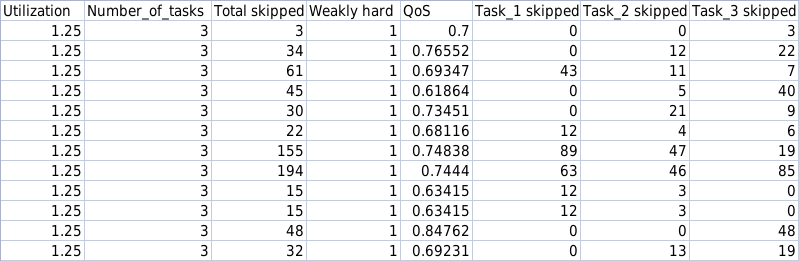
\includegraphics[width=\textwidth]
    {images/csv.png}}
    \caption{\label{fig:my-label} Primjer datoteke u koju se spremaju izvještaji simulacija}
  \end{figure}

\section{Pokretanje simulacije}

Pri pokretanju simulacije programu se preko argumenata prosljeđuju 3 parametra: broj zadataka, 
faktor opterećenja te naziv datoteke u koju će se upisivati izvještaj nakon završene simulacije.
Faktor opterećenja se radi jednostavnosti implementacije prosljeđuje pomnožen sa 100, jer bash ne podržava rad s decimalnim brojevima.

Za analizu rezultata potrebno je napraviti velik broj simulacija. Kako bi se taj proces automatizirao i ubrzao, implementirana 
je bash skripta \texttt{simulation.sh}. U skripti se zadaje naziv algoritma koji se trenutno koristi (koji je uključen u 
konfiguracijskoj datoteci). Pojedini algoritam potrebno je simulirati za faktore opterećenja u rasponu od 0.9 do 1.5 uz korake 0.05.
Kako bi se to ostvarilo, petljom se prolazi po svim faktorima opterećenja iz navedenog intervala. U svakoj iteraciji petlje stvara se datoteka tipa
csv, naziva oblika \texttt{{ime\_algoritma}\_{faktor\_opterećenja}.csv}. Na primjer, uz korištenje BWP algoritma i faktora opterećenja 1.25 
datoteka će se zvati \texttt{BWP\_125.csv}. Skripta će nadalje pokrenuti simulaciju sa zadanim faktorom opterećenja 20 puta te će se rezultati 
svake simulacije pohraniti u jedan redak navedene datoteke. Završetkom rada skripte generirano je 13 datoteka, a u svakoj se nalaze rezultati 
20 simulacija. Simulaciju je potrebno posebno pokrenuti za svaki ispitivani algoritam. U nastavku je prikazan pseudo kod skripte \texttt{simulation.sh}: 


\begin{lstlisting}[style=CStyle,caption={Pseudo kod skripte \texttt{simulation.sh}},captionpos=b]
zadavanje_algoritma;
for (i=90;i<=150;i+=5) do
	faktor_opterecenja=i;
	generiranje_imena_datoteke;
	stvaranje_datoteke_izvjestaja;
	for (j=0;j<20;j+=1) do
		pokretanje_simulacije(faktor_opterecenja,broj_zadataka,ime_datoteke);
	done
done
\end{lstlisting}

\end{document}